\documentclass[12pt,a4paper,openright,twoside]{book}
\usepackage[utf8]{inputenc}

\newcommand{\thesislang}{italian}
\usepackage{thesis-style}

\title{
    Ascent Essentials \\
    \large Applicazioni e Servizi Web
}

\author{Filippo Vissani - 0001026702 filippo.vissani@studio.unibo.it}
\date{19 Gennaio 2024}

\usepackage{natbib}
\usepackage{graphicx}

\begin{document}

\maketitle
\chapter{Introduzione}
Nel panorama sempre crescente dell'e-commerce, la necessità di fornire piattaforme specializzate che soddisfino le esigenze di comunità specifiche è diventata cruciale. In questo contesto, presentiamo il progetto "AscentEssentials", un E-Commerce dedicato agli appassionati delle attività sportive in montagna. La nostra missione è offrire una piattaforma completa e intuitiva che soddisfi le esigenze degli amanti dell'arrampicata, dell'alpinismo e del trekking, fornendo loro un accesso agevole a attrezzature e accessori di alta qualità.

Il team di "AscentEssentials", composto da Filippo Vissani ed Eddie Barzi, ha lavorato diligentemente per sviluppare un ambiente online che non solo semplifichi il processo di acquisto, ma che crei anche una comunità dedicata di appassionati. Attraverso una vasta gamma di funzionalità, il nostro obiettivo è rendere l'esperienza di acquisto non solo efficiente ma anche arricchente, fornendo ai nostri clienti un luogo virtuale in cui possono esplorare, acquistare e condividere la loro passione per le attività all'aria aperta.

Nel corso di questa relazione, esploreremo dettagliatamente le funzionalità chiave di "AscentEssentials", evidenziando le scelte di progettazione, le sfide affrontate e le soluzioni implementate per fornire un servizio all'altezza delle aspettative degli utenti. Da un catalogo ben curato a un sistema di checkout sicuro e intuitivo, ogni aspetto del progetto è stato attentamente considerato per garantire un'esperienza senza soluzione di continuità per gli acquirenti e i commercianti.

Siamo entusiasti di presentare "AscentEssentials" come una risorsa affidabile e coinvolgente per la comunità degli sportivi in montagna, contribuendo a connettere gli appassionati e fornendo loro gli strumenti necessari per esplorare e perseguire le proprie passioni. Iniziamo il nostro viaggio attraverso le funzionalità e le sfide affrontate in questa avventura di e-commerce specializzato.

\chapter{Requisiti}
Descrizione delle caratteristiche e funzionalità che il sistema prevede. 

\chapter{Design}
Design dell'architettura del sistema e delle interfacce utente.

\begin{figure}[h!]
\centering
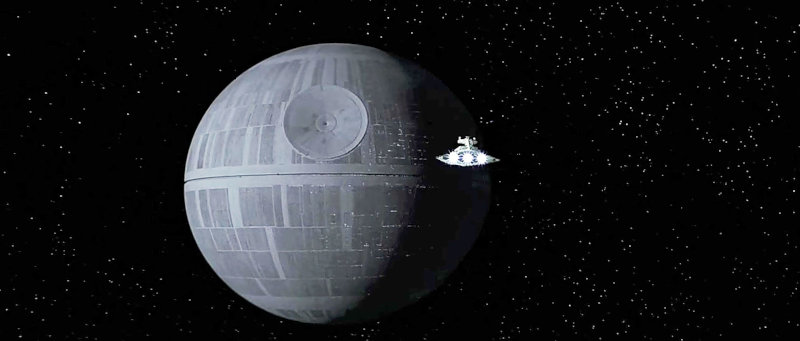
\includegraphics[scale=0.44]{deathStar2.jpg}
\caption{Death Star}
\label{fig:deathstar}
\end{figure}

\chapter{Tecnologie}
Tecnologie adottate e motivazioni.

\chapter{Codice}
Solo aspetti rilevanti.

\chapter{Test}
Test effettuati sul codice e test con utenti.

\chapter{Deployment}
Rilascio, installazione e messa in funzione.


\chapter{Conclusioni}
Conclusioni

\bibliographystyle{plain}
\bibliography{references}
\end{document}
